\documentclass{assignment}
\urlstyle{same}

\usepackage{listings} 
\let\verbatim\undefined 
\let\verbatimend\undefined 
\lstnewenvironment{verbatim}{\lstset{breaklines,basicstyle=\ttfamily}}{}
\linespread{1.5}

\author{Leigh Goetsch}
\prof{Dr. Turney}
\className{Systems Programming}
\classCode{CPE 2600}

\submissionDate{11/25/2024}
\title{Lab 11: Multiprocessing} 

\begin{document}
\maketitle
% \begin{multicols}{2}
% \raggedcolumns

\newpage

% In the report, include:
% a. A brief overview of your implementation.
% b. The graph of your runtime results. You will need to export the plot (from Excel) into an image, add the image to your repo, and then link it into the README.md.
% c. A brief discussion of your results.

\section{Overview}

I implemented the movie program and benchmarking program by modifying the \verb|mandel.c| program to have a method called \verb|fly_in()|. This takes the same arguments as \verb|mandel()|, but updates the \verb|center| and \verb|zoom| values to fly into the fractal. The \verb|fly_in()| method is called in a loop in the \verb|main()| method to create a movie of the fractal.

The \verb|mandelmovie| program takes most of the same arguments as \verb|mandel|, but also takes a \verb|num_children| argument (\verb|-n| default to 1) to specify the number of children to fork. The parent process will call \verb|fly_in()|, and the children will call \verb|mandel()| to render the fractal. The parent process will wait for all children to finish before updating the fractal and rendering the next frame.

The \verb|benchmark| program goes through the list [1, 2, 5, 10 20] for the number of children to fork, and runs the \verb|fly_in()| method with the specified number of children. The program records the time it takes to render the fractal for each number of children, and outputs the results to a CSV file, then graphs the results using \verb|gnuplot|.

\section{Results}

Here is the table of results from the benchmark program:
\begin{table}
    \centering
    \begin{tabular}{ll}
	\toprule
	num\_children & runtime \\
	\midrule
	1 & 397.798254 \\
	2 & 212.495177 \\
	5 & 101.662532 \\
	10 & 61.160311 \\
	20 & 59.847350 \\
	\bottomrule
    \end{tabular}
    \caption{Benchmark results}
\end{table}

The graph of the results:

\begin{figure}
    \centering
    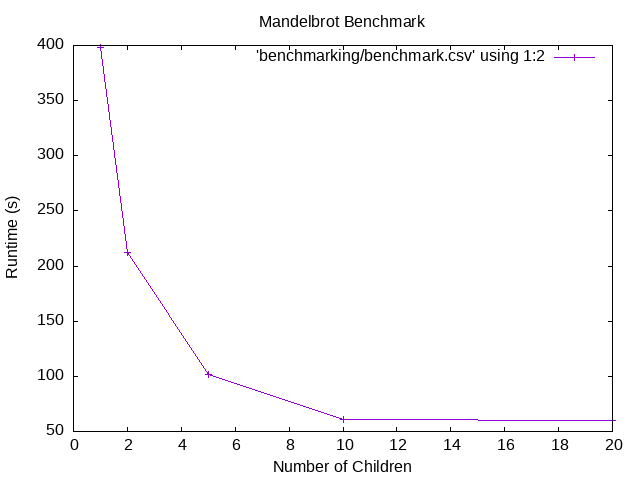
\includegraphics[width=0.8\linewidth]{images/benchmark.png}
    \caption{Benchmark results}
\end{figure}

The graph shows that runtime decreases as the number of children increases, which is expected since children render the fractal in parallel. The runtime drops significantly from 1 to 2 children and then decreases more gradually with additional children.


% \end{multicols}
\end{document}